\documentclass{article}

\title{Static types are for perfectionists}
\subtitle{Scherzo in e-moll on programming and authenticity.}
\date{2025-04-01}
\modified{2025-04-01}

\begin{document}
\section*
\epigraph{
  If you're making games, you should be getting therapy.
}{Mike Acton on the \href{https://youtu.be/rW1KMO2O6ak?si=GYOgrDPfKVGAbUJ_&t=2938)}{Wizardology podcast}}

In this article, I reflect on my professional preferences and trace them to my early childhood experiences.
I argue that culture and upbringing shape our core beliefs about technology more than rational arguments.
I conclude with two implications of this idea:
the necessity to accept other people's preferences without judgment and the importance of finding an environment rewarding your style.

\section{technology-mirror}{The technology mirror}

\epigraph{
  Perhaps the most decisive element of my game was the way my style on the board was completely in synch with my personality as a child.
}{Josh Waitzkin, ``The Art of Learning''}

For most of my programming career, I believed that my technological preferences were rational and reflected the realities of software development.
I thought people who disagreed with my views hadn't seen the light and hadn't felt the pain yet.
Give them time and relevant experience, and they will arrive at the same conclusions:
\begin{itemize}
\item
  Statically typed languages are the only way to do serious software development.
\item
  Programmers must grok and have a solid mental model of their systems.
\item
  Dependencies are evil.
  They complicate infrastructure and deployment and slow down development in the long run.
\end{itemize}

A few years ago, after reading half a library worth of books on personal development and psychology,
I realized how profoundly my early years affected my relationships, values, and core beliefs.
In particular, the following two traits of my formative years stood out:

\begin{itemize}
\item
  Mistakes were costly.
  Breaking something or getting a bad grade at school could result in punishment.
  As a result, my brain wants to avoid (or at least hide) mistakes.
  It demands perfection.
\item
  Asking for help, even from parents, often resulted in humiliation.
  As a result, I became \href{https://en.wikipedia.org/wiki/Counterdependency}{counterdependent}.
  Seeking or accepting help feels daunting.
  I'd rather read a gazillion books on psychology than talk to a therapist.
\end{itemize}

It didn't take me long to realize that my technology preferences mirrored my everyday behavior.
Thus, my early conditioning is a better explanation for my choices than objective evaluation:

\begin{itemize}
\item
  I prefer compiled languages because they help me avoid mistakes.
  My disdain for mistakes guides my interest in type systems, compilers, and formal methods.
  These tools make me feel safe\sidenote{sn-type-system-effectiveness}{
    That's a warm fuzzy feeling.
    There is \href{https://danluu.com/empirical-pl/}{little empirical evidence} that strong type systems lead to better programs.
  }.
\item
  Groking my programs reduces my dependence on tools and people.
  It also helps me fix bugs since I can simulate the system behavior in my head.
\item
  Eliminating dependencies gives me a sense of control and improves iteration time.
  If my code needs adjustments, I can make them without involving others or waiting for upstream fixes.
  In addition, having all the code in one place makes programming tools more reliable.
\end{itemize}

Does my conditioning help me write better programs? Maybe.
I noticed that my obsession with understanding leads to programs with few bugs,
most of which come not from internal inconsistencies but from incorrect assumptions about the execution environment.
Dependency aversion speeds up building, packaging, and shipping.

Do I prefer my approach \emph{because} it produces better programs? Probably not.
I can rationalize it all day long,  but in the end, it boils down to feelings.
Spending an hour fighting the compiler to craft a program that works on the first run feels terrific.
Spending twenty minutes on drafting a Python script and another twenty on squeezing out runtime bugs\ldots  doesn't.

I met many people whose programming approach was my polar opposite.
They threw stuff together, experimented, and pulled in behemoth frameworks.
They stopped worrying when their programs seemed to work and moved on.
I don't have any issues with their way, as long as we don't work on the same system.
In the long run, these builders might bring more value to the world than me.
They fear less and try more.

\section{authenticity-spiral}{The authenticity spiral}

\epigraph{
  In the beginner's mind there are many possibilities, but in the expert's there are few.
}{
  Shunryu Suzuki, ``Zen Mind, Beginner's Mind: Informal Talks on Zen Meditation and Practice''
}

Of course, I didn't enter the profession as a fully-formed lonely grumbler.
My views evolved significantly throughout my career, and continue to change.

My first programs were physics simulations and tiny games in \href{https://en.wikipedia.org/wiki/Turbo_Pascal}{Turbo Pascal}.
They were dull and brutally direct.
I would create animations by individually drawing pixels at specific offsets.
My only dependency was the standard library.

When I became a junior engineer in Enterprise Java world, I became obsessed with clean code.
I read every book on code organization, packed my code with design patterns, and mastered bloated frameworks.

Exposure to new ideas and programming languages made me realize that most things I considered good design were unnecessary.
They didn't contribute to the solution but created accidental complexity and bloat.
I didn't need to write extensible code.
I could start with the most straightforward version and rewrite it when the problem changed.
As \href{https://programmingisterrible.com/about}{tef} puts it, \href{https://programmingisterrible.com/post/139222674273/write-code-that-is-easy-to-delete-not-easy-to}{code should be easy to delete}.

It took me over a decade to distill a programming style that resonated with me.
I now care little about abstract clean code conventions and use my aesthetics and feelings as guides.
That tendency sometimes leads to communication problems: I often \emph{feel} that one design is preferable but can't explain why exactly.

As all artists, programmers grow in spirals.
Beginners try to achieve goals in the most straightforward way they know.
Every line of code they write serves a purpose. Then they learn paradigms and ``good practices'' and imitate them.
They accept that things must be done in a particular way because that's the way of the craft.
This path leads them astray, but it's necessary for growth.
They exit this limbo by reconnecting with reality and returning to their \href{https://en.wikipedia.org/wiki/Shoshin}{beginner's mind}.
Their code becomes simple and purposeful again.
Conventions fade, and their work becomes more authentic.

\begin{figure}[medium-size,grayscale-diagram]
\marginnote{mn-auth-spiral}{
    Programmers grow in spirals.
    Beginners think intuitively, but lack the language to express themselves.
    As they acquire knowledge and imitatate others, they curve away from their core in the authenticity space.
    Eventually, they learn to see things clearly and become more authentic.
}
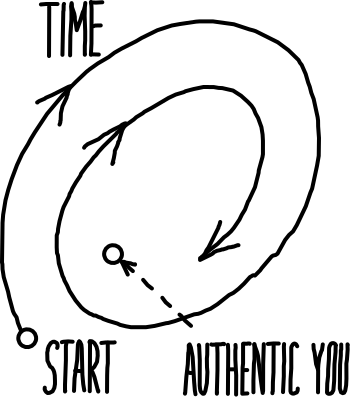
\includegraphics{/images/38-auth-spiral.svg}
\end{figure}

The Japanese martial arts concept of \href{https://en.wikipedia.org/wiki/Shuhari}{shuhari} describes three stages of mastery;
it maps well to the authenticity spiral:
\begin{enumerate}
\item At the \emph{shu} stage, the practitioner learns the fundamentals, memorizes the moves, and obeys the rules.
That's the upward curve on the spiral.
\item At the \emph{ha} stage, the practitioner starts innovating by breaking the rules and connecting with reality.
That's the backward trend on the spiral.
\item At the \emph{ri} stage, the practitioner transcends the forms and performs the moves naturally.
By this stage, the spiral approaches the authentic core.
\end{enumerate}

If your views on technology don't resonate with your core beliefs in other areas of life,
your spiral might not have completed its cycle yet.

\section{finding-your-place}{Finding your place}

\epigraph{
You will excel only by maximizing your strengths, never by fixing your weaknesses.
}{Marcus Buckingham}

Let's say I convinced you that your technological preferences result mostly from your upbringing and culture.
What are the implications? I can think of at least two.

Firstly, we should stop labeling and accusing people who don't share our preferences.
Using a memory-unsafe language isn't a moral crime, and a preference for dynamic typing doesn't say anything about the programmer's intelligence.
Type theory maximalists should give up their aura of moral and intellectual superiority and accept that they need therapy just as badly as everyone else in the industry (if not more).

\begin{figure}[medium-size]
\marginnote{mn-galois-credit}{
  The sleep of self-awareness produces elegant mathematical constructs.
  \newline
  Source: \href{https://x.com/LongFormMath/status/1526564036405391361}{Jay Cummings}.
}
\center{
  
\includegraphics{/images/38-galois.jpg}
}
\end{figure}

Secondly, we should pay more attention to how the technology feels and incorporate these feelings in our career choices.

Environment plays a crucial role in productivity and job satisfaction.
I experienced this firsthand as my productivity fluctuated throughout my career.
I felt at home and very productive at Yandex.Maps, and my managers were pleased with my work.
When I joined Google, I felt like a cog in a vast machine.
My motivation and productivity plummeted; I found it hard to focus and advance my projects.
Joining \textsc{dfinity} and building things from the ground up was thrilling and stimulating; my four-and-a-half years there were the most productive in my life.
I thought this experience changed me for good and gave me wings.
I thought I could handle anything that landed on my plate.
Yet, my productivity vanished after I left \textsc{dfinity} and joined an oversized startup.
In just a few months, I felt burnt out and useless.
And then it dawned on me that I didn't change much between my experiences.
My environment influenced my motivation and productivity much more than my track record.
I need the right project and the right team to function well\sidenote{sn-productivity-books}{
  Most productivity books, including \href{https://www.goodreads.com/book/show/1633.Getting_Things_Done}{Getting Things Done} and \href{https://www.goodreads.com/book/show/10009377-the-12-week-year}{The 12 Week Year},
  promise you that their system will turn you into a productivity machine no matter what life throws at you. They lie.
}.

The right environment doesn't make everything easy.
You'll still be frustrated a lot and will face challenges.
But getting through these challenges will feel like growth, not a drag.
Hence, understanding what makes you tick and finding a place where you belong (not a place where \emph{you think you should belong}) will make you happier.

\section{final-words}{Final words}

\epigraph{
  Haskell will still be used in 20 years,
  because there will always be people looking for a productive way to weaponize their autism.
}{\href{https://x.com/effectfully/status/1901124439258894769}{@effectfully}}

Unfortunately, I couldn't find any research that could disprove or confirm my anecdotal observations.
If you're a researcher working in the intersection of psychology and computer science, consider investigating the effects of childhood experience and neurodiversity\sidenote{sn-haskell-nd}{
  As a frequent \href{https://zfoh.ch/zurihac2024/}{ZuriHac} guest,
  I got an impression that hard-core compiled language communities have an unusually large fraction of neurodiverse people.
} on technology preferences.
I can't wait to read your papers!

If you liked this article,
consider listening to the \href{https://corecursive.com/leaving-stripe-with-jon-de-le-motte/}{Leaving Stripe} episode of the \href{https://corecursive.com/}{CoRecursive} podcast.
In this episode, Jon de la Motte shares his struggles with mental health and connects his career choices to his family dynamics.

I'm waiting for my first therapy appointment.
Don't hesitate to book one, too.

\end{document}